\documentclass{amsart}

% === PACKAGES === (((
\usepackage{amsmath}
\usepackage{amsfonts}
\usepackage{amssymb}
\usepackage{graphicx}
\usepackage{mathrsfs}
% )))

% === TITLE === (((
\title{On Transformations Between Symmetric Spaces.}
\keywords{Metric spaces, symmetric spaces, transformations, mappings}
% )))

% === AUTHORS === (((
%    author one information
\author{Erick I. Rodríguez Juárez.}
\address{Aguascalientes. Ags}
\curraddr{20174, Mexico}
\email{nijerc@gmail.com}
% \thanks{Jorge Macías Díaz.}

%    author two information
\author{Jorge E. Macías Díaz.}
\address{Aguascalientes. Ags}
\curraddr{Mexico}
\email{jemacias@correo.uaa.mx}
% \thanks{}
\subjclass[2010]{Primary }
% )))

% === ENVIRONMENTS === (((
\newtheorem{theorem}{Theorem}[section]
\newtheorem{lemma}[theorem]{Lemma}
\newtheorem{corollary}[theorem]{Corollary}

\theoremstyle{definition}
\newtheorem{definition}[theorem]{Definition}
\newtheorem{example}[theorem]{Example}
\newtheorem{xca}[theorem]{Exercise}

\theoremstyle{remark}
\newtheorem{remark}[theorem]{Remark}

\numberwithin{equation}{section}
% )))

% === COMMANDS === (((
\newcommand{\dis}{\displaystyle}
% )))

\begin{document}

% === ABSTRACT === (((
\begin{abstract}
	We consider the concept proposed by \cite{feng}.
\end{abstract}
\maketitle
% )))

\section{Isometries of Symmetric Spaces.} % (((
\begin{definition}
	Let \(X\) be a set. We say that \((X,d)\) is a \textbf{metric space} if \(d:X^2 \longrightarrow \mathbb{R}\) satisfies:
	\begin{enumerate}
		\item \(d(x,y) =0 \iff x = y\).
		\item \(d(x,y) = d(y,x)\), \(\forall x,y \in X\).
		\item \(d(x,y) \leqslant d(x,z) + d(z,y)\), \(\forall x,y,z \in X\).
	\end{enumerate}
\end{definition}
\begin{definition}
	Let \((X,d)\) and \((Y,d')\) be metric spaces.
	We say that a function \(f:X \longrightarrow Y\) is an \textbf{isometry} if \(d(x,y) = d' (fx,fy)\), \(\forall x,y \in X\).
	In that case, \(X\) and \(Y\) are \textbf{isometric}.
\end{definition}
\begin{definition}
	Let \(X\) be a metric space. \\
	\begin{minipage}{0.7\linewidth}
		We say that \(X\) \textbf{is \(x_0-\)symmetric with the map \\\(f:X \longrightarrow X\)} if
		\begin{enumerate}
			\item \(f\) is an isometry.
			\item \(d(x,x_0) = d(fx,x_0) = \dfrac{1}{2} d(x,fx)\), \(\forall x \in X\).
		\end{enumerate}
	\end{minipage}
	\begin{minipage}{0.3\linewidth}
		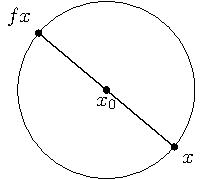
\includegraphics[width= 0.9 \linewidth, page = 1]{IMAGENES/1/tikz.pdf}
	\end{minipage}
	In that case, if there is no ambiguity, we say that \(X\) is a \textbf{\(x_0-\)symmetric space}.
\end{definition}
Every isometry is biyective, and its inverse is also an isometry.
The composition of isometries is an isometry.
\begin{theorem}
	If \((X,d)\) is \(x_0\)-symmetric with \(f\), then \(X\) is \(x_0\)-symmetric with \(f^{-1}\).
\end{theorem}
\begin{theorem}
	Let \((X,d), (Y,d')\) be metric spaces.
	Let \(X\) be a \(x_0-\)symmetric space with \(f\).
	Let \(\varphi :X \longrightarrow Y\) be an isometry.
	Then \(Y\) is a \(\varphi x_0-\)symmetric space with \(g = \varphi \circ f \circ \varphi ^{-1}\).
\end{theorem}
\begin{proof}
	\begin{enumerate}
		\item \fbox{\(g\) is an isometry}
			\[
				d' (gx,gy) = d' (\varphi f \varphi ^{-1} x \;,\; \varphi f \varphi ^{-1} y) = d'(x,y).
			\]
		\item \fbox{\(d' (x, \varphi x_0) \stackrel{(a)}{=} d' (gx, \varphi x_0) \stackrel{(b)}{=} \dfrac{1}{2} d' (x,gx)\), \(\forall x \in Y\)}.
			\begin{enumerate}
				\item \(\)
					\[
						\begin{array}{rcl}
							d' (gx, \varphi x_0) & = & d' (\varphi f \varphi x, \varphi x_0) \\[2mm]
							& = & d(f \varphi ^{-1} x, x_0) \\[2mm]
							& = & d(\varphi ^{-1} x,x_0) \\[2mm]
							& = & d' (x, \varphi x_0).
						\end{array}
					\]
				\item 
					\[
						\begin{array}{rcl}
							\dfrac{1}{2} d'(x,gx) & = & \dfrac{1}{2} d' (x, \varphi f \varphi ^{-1} x) \\[2mm]
							& = & \dfrac{1}{2} d(\varphi ^{-1} x, f \varphi ^{-1} x) \\[2mm]
							& = & d(f \varphi ^{-1} x, x_0) \\[2mm]
							& = & d' (\varphi f \varphi ^{-1} x, \varphi x_0) = d' (gx, \varphi x_0).
						\end{array}
					\]
			\end{enumerate}
	\end{enumerate}
\end{proof}
\begin{example}
	If \((X,d)\) is symmetric to \(x_0\) with \(f\) and \(g\), then no necessarily \(X\) is symmetric to \(x_0\) with \(f \circ g\).
	Consider \(X = \mathbb{R}\) with \(d(x,y) = |x-y|\), and \(f = g: \mathbb{R} \longrightarrow \mathbb{R}\) defined by \(f(x) = -x\). Then
	\begin{enumerate}
		\item \(f\) is an isometry.
		\item \(d(x,0) = d(fx,0) = \dfrac{1}{2} d(x,fx)\).
	\end{enumerate}
	But \(f \circ f = I\), the identity map, it's not a symmetric function to the space, since \(\dfrac{1}{2} d(x, f \circ fx) = 0\), \(\forall x \in X\).
\end{example}
% )))

\section{Subspaces.} % (((
\begin{corollary}
	Let \((X,d)\) be a\(x_0-\)symmetric space with \(f\).
	Let \(A \subseteq X\), and \(a \in A\).
	If \(A\) is \(a-\)symmetric space with \(g\), then \(f(A)\) is \(f(a)-\)symmetric with \(g':f(A) \longrightarrow f(A)\), by \(g' = f \circ g \circ f^{-1}\).
\end{corollary}
\begin{proof}
	It follows from the fact that \(A\) and \(f(A)\) are isometric.
\end{proof}
\begin{definition}
	Let \((X,d)\) be a metric space, and \(A,B \subseteq X\).
	Let \(x \in A\).
	We define \(d(x,A) = \dis \inf _{y \in A} d(x,y)\), and
	\[
		d(A,B) = \inf _{\substack{x \in A \\ y \in B}} d(x,y). 
	\]
\end{definition}
It's easily seen that \(d(A,B) = \dis \inf _{y \in B} d(y,A)\).
\begin{theorem}
	Let \(X,d\) be a \(x_0-\)symmetric space with \(f\).
	Let \(A \subseteq X\).
	Then
	\[
		d(A,x_0) = d(f(A) , x_0) = \dfrac{1}{2} d(A,f(A)).
	\]
\end{theorem}
\begin{proof}
	\begin{enumerate}
		\item \fbox{\(d(A,x_0) = d(f(A) ,x_0)\)} Since \(f\) is a biyection, we have
			\[
				d(f(A) ,x_0) = \inf _{y \in f(A)} d(y,x_0) = \inf _{x \in A} d(fx,x_0) = \inf _{x \in A} d(x,x_0) = d(A,x_0). 
			\]
			% First, we see that
			% \[
				% \dfrac{1}{2} \inf _{x \in A} d(x,fx) = \inf _{x \in A} d(fx,x_0) = \inf _{y \in f(A)} d(y,x_0) = d(f(A) ,x_0).
			% \]
			% And the following inequalities.
			% \[
				% \inf _{x \in A} d(x,fx) \geqslant \inf _{\substack{x \in A \\ y \in f(A)}} d(x,y) = d(A,f(A)).
			% \]
			% Then
			% \[
				% d(f(A) ,x_0) = \dfrac{1}{2} \inf _{x \in A} d(x,fx) = \dfrac{1}{2} d(A,f(A)).
			% \]
		\item \fbox{\(d(f(A) ,x_0) = \dfrac{1}{2} d(A,f(A))\)} Since \(f\) is a biyection
			\[
				d(f(A) ,x_0) = \inf _{x \in A} d(fx,x_0) = \dfrac{1}{2} \inf _{x \in A} d(x,fx) \geqslant \dfrac{1}{2} \inf _{\substack{x \in A \\ y \in f(A)}} d(x,y) = \dfrac{1}{2} d(A,f(A)).
			\]
			And, we notice that
			\[
				d(fx,x_0) = \dfrac{1}{2} d(x,fx) \leqslant \dfrac{1}{2} \big[d(x,y) + d(y,fx)\big], \hspace{5mm} \forall x \in A \;,\; y \in f(A).
			\]
			Then
			\[
				\begin{array}{rcl}
					d(f(A) ,x_0) = \dis \inf _{x \in A} d(fx,x_0) & \leqslant & \dfrac{1}{2} \dis \inf _{\substack{x \in A \\ y \in f(A)}} \big[d(x,y) + d(y,fx)\big] \\[5mm]
					& = & \dfrac{1}{2} \dis \inf _{\substack{x \in A \\ y \in f(A)}} d(x,y) \hspace{5mm} (\forall y \in f(A) \;,\; \exists x \in A \;:\; fx = y)\\[5mm]
					& = & \dfrac{1}{2} d(A,f(A)).
				\end{array}
			\]
			So \(d(f(A) ,x_0) = \dfrac{1}{2} d(A,f(A))\).
	\end{enumerate}
\end{proof}
TODO:
\begin{enumerate}
	\item \(X\) is bounded (\((B(x_0,r) = X)\)). Define \(d(f,g) = \dis \sup _{x \in X} d(fx,gx) \). What happens if \(g=I\).
	\item diameter
	\item orbit of \(f\).
	\item Properties of \textit{the Hausdorff metric} \(\delta : \mathscr{P} (X) ^2 \longrightarrow \mathbb{R} \), defined by
		\[
			\delta (A,B) = \max \{\dis \sup _{x \in A} d(x,B) \;,\;  \dis \sup _{y \in B} d(A,y)\}.
		\]
\end{enumerate}
% )))

\section{Completion.} % (((
\begin{definition}
	Let \((X,d)\) be a metric space, and \(A \subseteq X\).
	We define \(cerrA = \{x \in X \;:\; d(x,A) =0\}\).
	We say that \(A\) \textbf{is dense on \(X\)}, if \(cerrA = X\).
\end{definition}
\begin{definition}
	We say that a metric space \((X,d)\) is \textbf{complete} if every Cauchy sequence of \(X\) converges on \(X\).
\end{definition}
% \begin{theorem}
	% Let \((X,d)\) be a metric space.
	% Let \(B_\mathbb{R} (X) = \{f: X \longrightarrow \mathbb{R} \;|\; f \mbox{ is bounded}\}\), and
	% \(d'(f,g) = \sup _{x \in X} d(fx,gx)\).
	% Then \((B_\mathbb{R} (X) , d')\) is complete.
% \end{theorem}
\begin{definition}
	Let \((X,d)\) be a metric space.
	We say that a metric space \((Y,d')\) is \textbf{a completion of} \((X,d)\) if 
	\begin{enumerate}
		\item \(Y\) is complete.
		\item \(\exists \varphi :X \longrightarrow Y\) isometry.
		\item \(\varphi (X) \subseteq Y\) is dense.
	\end{enumerate}
\end{definition}
\begin{theorem}
	Every completion of a symmetric space is symmetric.
\end{theorem}
% \begin{theorem}
	% There is a completion for every metric space.
% \end{theorem}
% )))

\section{Mappings Between Two Symmetric Spaces.} % (((
% )))

\section{Pairs of Symmetric Spaces.} % (((
% )))

\section{Path Metric Spaces.} % (((
\[
	dil(f) = \sup _{x \ne y} \dfrac{d(fx,fy)}{d(x,y)}.
\]
\[
	dil_x(f) = \dis\lim_{\varepsilon\rightarrow 0} dil(f \big| _{B(x, \varepsilon)}).
\]
The lentgh of a function \(f:A \subseteq \mathbb{R}^n \longrightarrow \mathbb{R} ^n\):
\[
	\ell (f) = \dis\int _A dil_x(f) dx.
\]
\[
	\beta (x,t) = \dis \inf _P \left\{t^{-1} \dis \sup _{y \in E \cap B(x,t)} d(y,P)\right\}.
\]
% )))

% === REFERENCES === (((
\bibliography{Referencias}
\bibliographystyle{amsplain}
% )))

\end{document}
